\section{Evaluation}
To evaluate our scheduling algorithm we are comparing the performance of Apache Cassandra (version 1.1.6)~\cite{Lakshman:2010:CDS:1773912.1773922} with and without our query assignment algorithm. We have chosen to use Cassandra because it is an open-source key-value database with a large community and is used by several enterprise clients~\cite{DataStaxCassandra}. To evaluate the performance of each version of Cassandra we are using the Yahoo! Cloud Service Benchmark (YCSB)~\cite{Cooper:2010:BCS:1807128.1807152}. The remainder of this section will describe the experimental setup and the results of the experiments.

\subsection{Experimental Configuration}
Our experiments were performed on a 10-server cluster running Ubuntu Linux 12.04. Each server has a 6-core 2.3GHz processor and 16GB of main memory. The machines are all located in close proximity (latency did not prove to be an issue in the experiments).

The data in Cassandra was partitioned using the \textit{RandomPartitioner} (equivalent to Consistent Hash Partitioning~\cite{consistentHashPartitioning}). The data was therefore equally distributed between all 10 nodes in the cluster (the Master server contained data to be queried on, but this did not appear to result in the master being overloaded). The replication factor used in our database was three. The read consistency was set to \textit{one} (meaning that the read query only looks at a single replica to get a result).

The baseline method for assigning queries to nodes in a Cassandra cluster is the \textit{SimpleStrategy}. This method just assigns the query to the first replica in the ring. It should be noted that this method is only adequate for single data-center databases (which is the only situation we have tested). Cassandra offers other choices (e.g., a method for a database distributed over multiple data centers and for use with Amazon's EC2 cloud environment), but given our experimental hardware configuration we did not explore these methods.

YCSB is used to generate and insert the data for the experiments. All of the data is stored in a single database table. There are 10 values associated with each key, with each value being 100 bytes. We ran our experiments on databases with 10 million keys and 150 million keys (corresponding to 10GB and 150GB databases). This was done to examine the impact that Cassandra's key and row caching would have on Cassandra with and without our query assignment algorithm.

We ran two different kinds of workloads against Cassandra: a 100\% read workload, and a 100\% scan (multi-key read) workload. The read-heavy workload was used because reads are the most time consuming single-key operation, and likewise scans are the most time consuming operation overall. The maximum scan length was set to 1000 keys, with the distribution over that range being uniform.

The queries are generated dynamically conforming to a Zipfian distribution~\cite{Gray:1994:QGB:191843.191886} with a skew of 0.99. We chose to use a Zipfian distribution so that the workload would differ between machines in the cluster (thus making our scheduling algorithm more applicable). The YCSB clients were run from one of the machines in the cluster (not the master). This did not appear to have any effect on the performance of the query assignment algorithm. 

The performance is measured in terms of operations per second that are performed. This is the default method that YCSB provides to measure performance. The YCSB also offers the ability to set a target for the number of operations that should be performed per second (similar to deadlines on the queries). However, this method sets the same deadline for every query and is directly related to the throughput, so we have chosen to only examine throughput. Each experiment has been performed using 5, 10, 20, 50 and 100 parallel YCSB clients.

\subsection{Experimental Results}
In this section, the performance with and without the query assignment algorithm is compared in each graph; the dashed line is the performance of the baseline Cassandra and the solid line is the performance using our query assignment algorithm. The Cassandra cluster was restarted between every run. The results are averaged over 3 runs each.

A problem that arose somewhat often was issues of test environment consistency between experimental runs. That is, it is not entirely uncommon for a node to crash during operation. Initially, we did not examine the node status after each run, and therefore our initial results from the experiments could be quite skewed in favor of one method or the other. In addition, one of the nodes in the cluster did not have its time synchronized with the other nodes, resulting the schema disagreement issues that caused that particular node to drastically decrease its performance. After recognizing that this was causing skewed results we re-ran all of our experiments and took these issues into account.

\begin{figure*}[t]
\centering
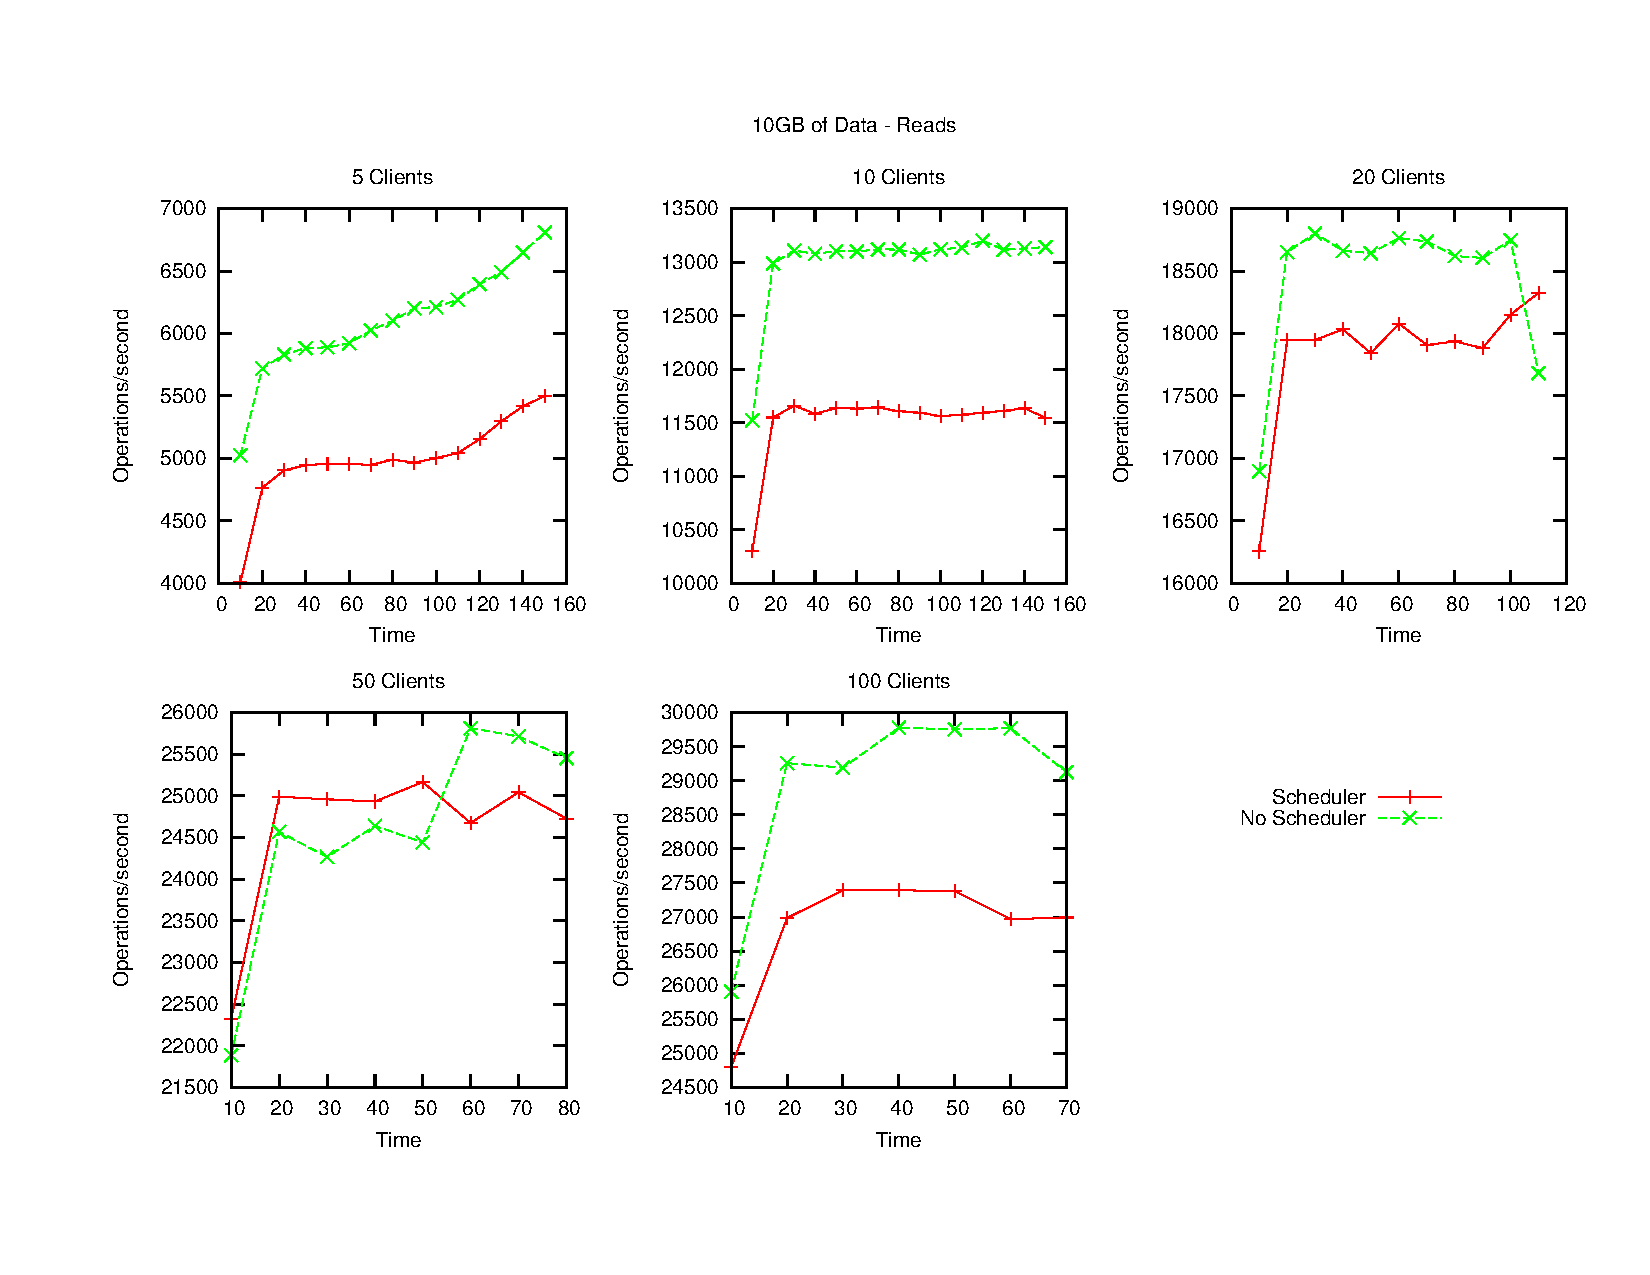
\includegraphics[scale=0.563]{images/10GB_Reads.pdf}
\vspace{-15pt}
\caption{The experimental results of performing the 100\% read workload on the 10GB database.}
\label{fig:10g_reads}
\end{figure*}

The results of the 10GB experiment are shown in Figure~\ref{fig:10g_reads}. As can be seen, the version of Cassandra using the resource based query assignment did not perform nearly as well as the baseline version. However, the difference in throughput between the scheduled and baseline versions tended to stay constant throughout the course of each experiment. As well, the ratio of the difference between experiments was very similar. This seems to indicate that the overhead of performing the additional assignment logic is what resulted in the decrease in performance. We also monitored the servers resource usage during the course of the experiment and found that the server was never heavily loaded, which means that the performance difference is very minor (i.e., there is no noticable difference between 10\% CPU usage and 12\% CPU usage).

\begin{figure*}[t]
\centering
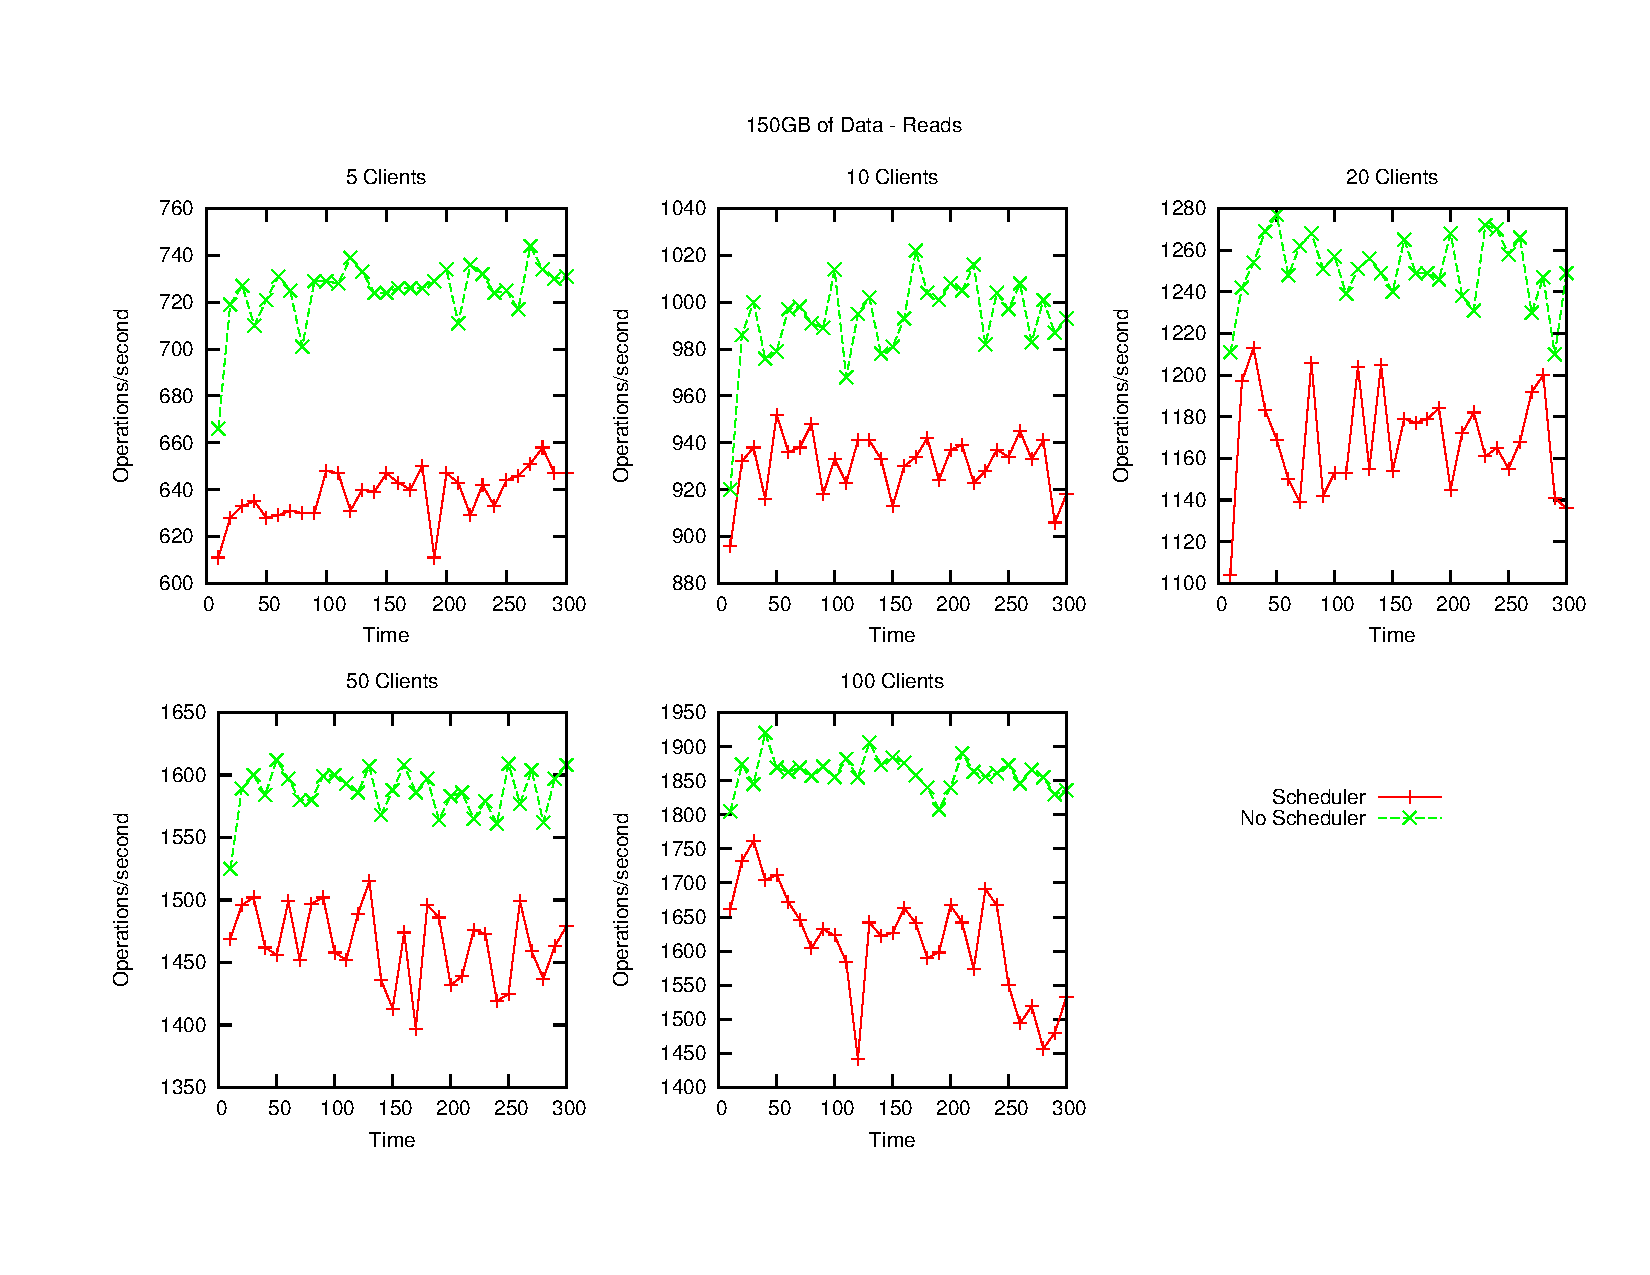
\includegraphics[scale=0.563]{images/150GB_Reads.pdf}
\vspace{-15pt}
\caption{The experimental results of performing the 100\% read workload on the 150GB database.}
\label{fig:150g_reads}
\end{figure*}

The results of running the 100\% read workload on a 150GB database are shown in Figure~\ref{fig:150g_reads}. As before, the scheduled version of Cassandra is slower than the baseline version in every case. The difference is performance is approximately 100 operations/second the 5, 10, 20 and 50 client experiments; the difference rises to over 150 operations/second in the experiment that uses 100 parallel clients.

We believe that the poor performance of the scheduling algorithm during the read workload is due to three reasons:

\begin{enumerate}

\item Even while 100 parallel clients were sending queries to the database, the node servers CPU usage and memory usage was very low. Therefore, the difference in throughput between the 150GB and 10GB databases (30000 operations/second versus 1900 operations/second) seems to indicate that hard-disk accesses are the bottleneck (this makes sense considering this is the bottleneck in traditional databases as well). This means that our resource usage formula is missing an important part of what determines how quickly a query can execute.

\item The introduced overhead of the scheduling logic seems to have a significant impact on our performance. This is especially apparent in the experiments on the 10GB database, where much of the data could be stored in the database cache. We believe that that this is what causes the throughput in the 10GB database experiments to differ by almost 1000 operations per second.

Unfortunately, this is not something that can be easily resolved. The baseline version of Cassandra does not perform any kind of analysis of the replica servers and instead just sends the query to the first replica. In our algorithm we are adding an additional thread and network calls to Cassandra, as well as scanning a vector of length $n$ (where $n$ = number of replicas) and finding the replica with the smallest resource value. In isolation these actions do not cause a noticeable drop in performance, but when performing 30000 reads per second there is significant overhead.

\item Another reason why the scheduled read could never have better performance than the unscheduled version is because of the use of read digests~\cite{readDigest} in Cassandra. A read digest is used to maintain consistency of replicas in the database. For every read query, Cassandra will read the value from the first replica, but also get a MD5 hash of the values on all of the other replicas. This is what Cassandra uses to gain eventual consistency. Naturally, a problem arises because even though we are reading the actual value from the least loaded replica, we are still querying the heavily loaded replicas to get a hash of the value.

It is for this reason that we have also examined how our assignment operation performs when applied to the scan operation (which does not perform a read digest).

\end{enumerate}

\begin{figure*}[t]
\centering
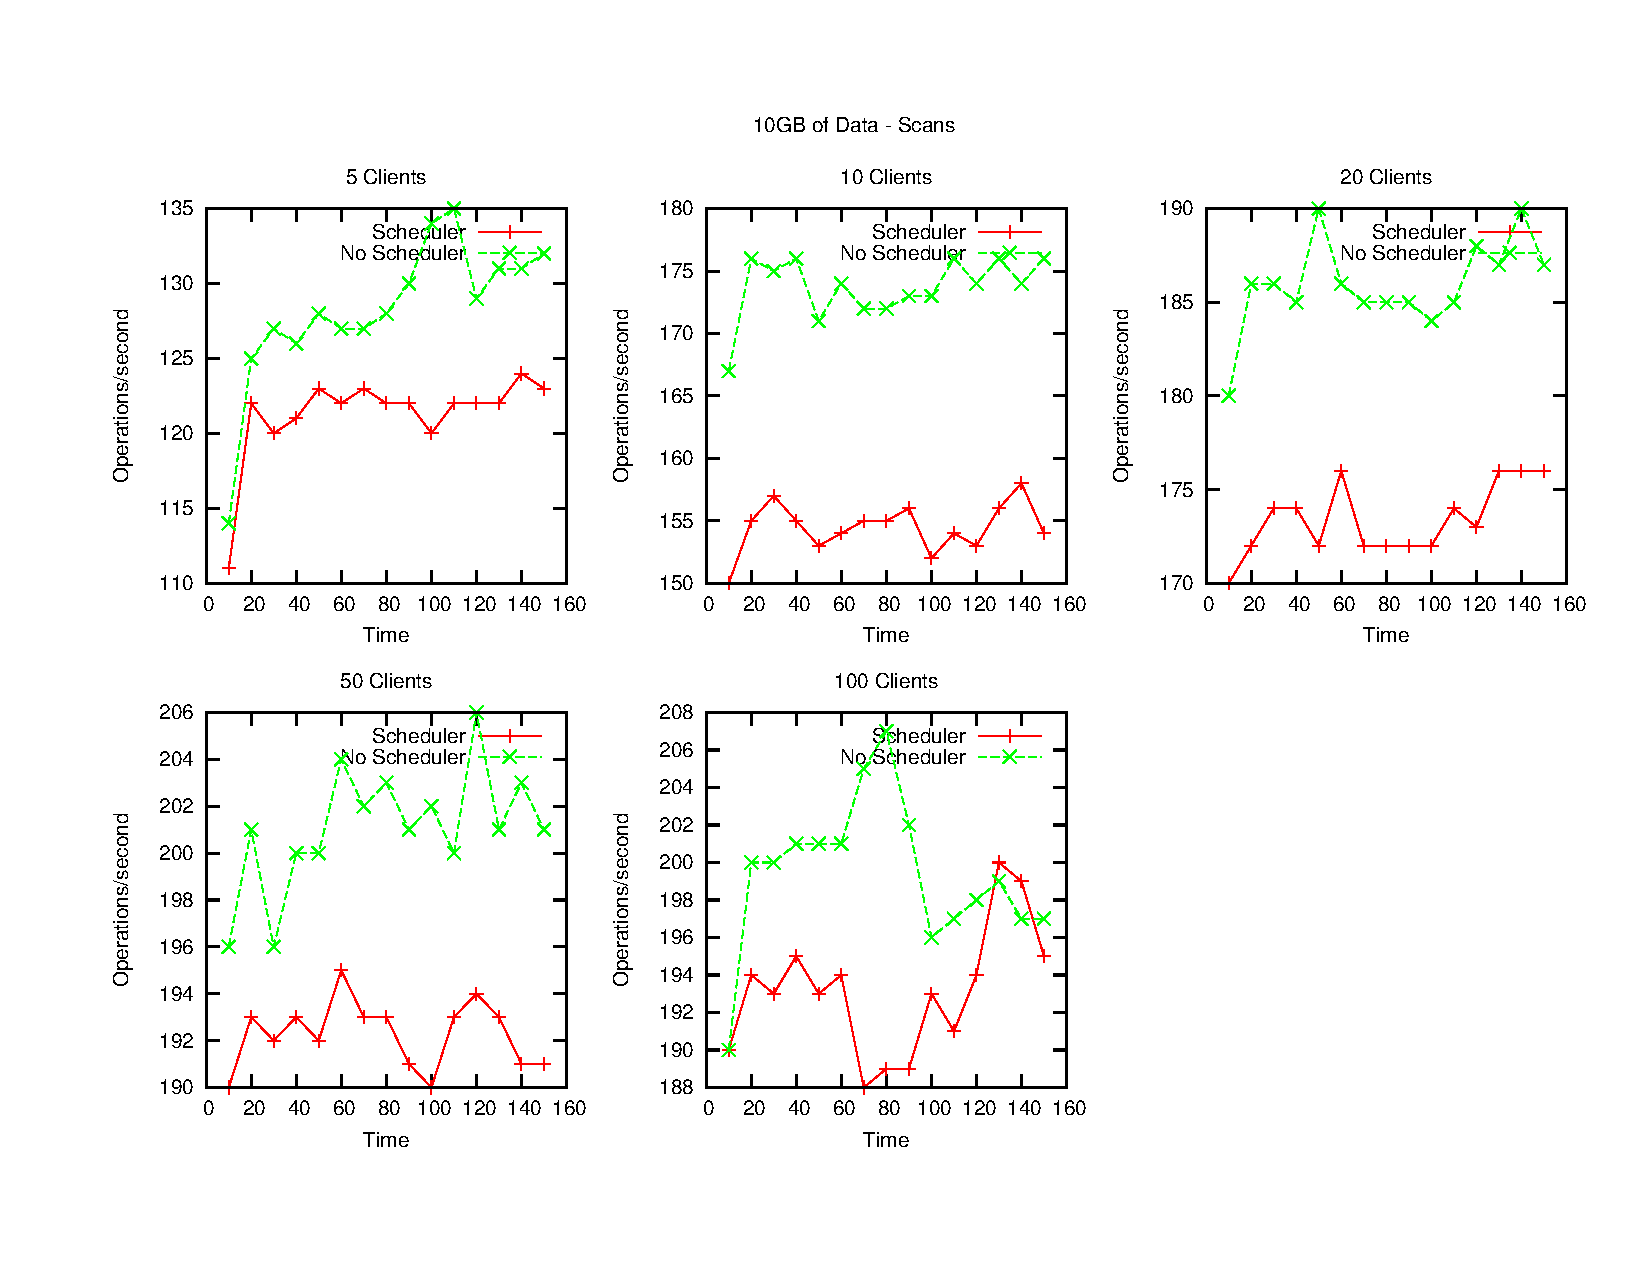
\includegraphics[scale=0.5]{images/10GB_Scans.pdf}
\vspace{-15pt}
\caption{The experimental results of performing the 100\% scan workload on the 10GB database.}
\label{fig:10g_scans}
\end{figure*}

The results of the scans experiment on the 10GB database are shown in Figure~\ref{fig:10g_scans}. In these experiments the performance of both versions of Cassandra are very close to one another. The results are particularly close for the experiments with 50 and 100 concurrent clients. We believe this is because when there are a high number of concurrent clients the CPU and memory usage varies enough between node servers that the query execution time is affected. We attempted to test with a greater number of clients than 100 (both 500 and 1000) and in both cases the results were similar because it appears that the master server became too heavily loaded.

Averaging the results of the experiments over 3 runs is not enough to say conclusively if the scheduled version of Cassandra provides better performance than the baseline version when performing scans with large numbers of concurrent clients. However, it appears that the performance of Cassandra when using the scheduling algorithm is at least on par with the performance of the baseline version of Cassandra. When the resource usage formula is improved to take factors other than CPU usage and memory usage into account it should, hopefully, provide consistently better performance than the baseline version of Cassandra. Confirming this requires further testing.

\begin{figure}[t]
\centering
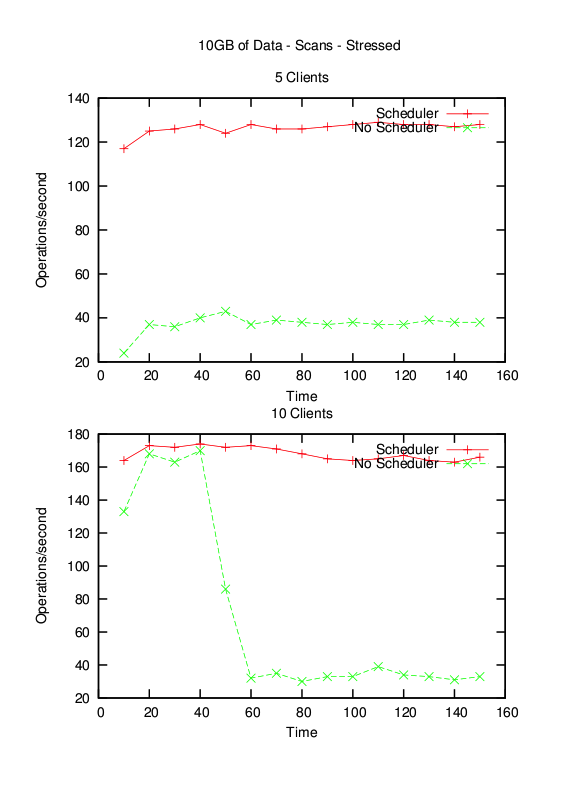
\includegraphics[scale=0.4]{images/10GB_Scans_Stressed.png}
\vspace{-15pt}
\caption{The experimental results of performing the 100\% scan workload on the 10GB database (where every second node is stressed).}
\label{fig:10g_scans_stressed}
\end{figure}

We also ran the 100\% scans workload on the 10GB database while introducing artificial CPU and memory work into the server (this was done using the stress\footnote{ http://weather.ou.edu/~apw/projects/stress/} tool). Every second node in the cluster was loaded by starting 30 processes that would continually malloc() and free() data. This resulted in fairly constant 100\% CPU and memory usage.

The results of the 5 and 10 client experiments are shown in Figure~\ref{fig:10g_scans_stressed}. In these cases you can see that the resource aware assignment has much better performance than the baseline Cassandra. This is because the resource aware assignment will consider that every second server is overloaded and not send queries to those servers. The results for the baseline version of Cassandra are taken from a single run of the YCSB. This is because the consequent runs all resulted in the YCSB throwing numerous exceptions before aborting. The figures for the cases with 20, 50 and 100 clients are not shown because performing experiments on the baseline version of Cassandra resulted in the YCSB benchmark continually aborting during the middle of the experiments. We believe this occurs because the queries sent to the heavily loaded server may be significantly delayed or lost, resulting in the YCSB believing the something is wrong with Cassandra (though we have not confirmed if this is actually the reason).

Although server load similar to the artificial load that we introduced may be quite rare in practice, we believe that this is the ideal environment to use our query assignment algorithm.